\documentclass[addpoints,11pt]{exam}

\usepackage{alltt}
\usepackage[margin=1in]{geometry}   % set up margins
\usepackage[T1]{fontenc}
\usepackage[usenames,dvipsnames]{xcolor}
\usepackage{enumerate}              % fancy enumerate
\usepackage{amsmath}                % used for \eqref{} in this document
\usepackage{amsthm}
\theoremstyle{definition}
\newtheorem{exmp}{Example}[section]
\usepackage{verbatim}               % useful for \begin{comment} and \end{comment}
\usepackage{eurosym}                % used for euro symbol
\usepackage{caption} 
\usepackage{graphicx}
\graphicspath{{Figures/}}
\usepackage{subcaption}
\usepackage{color}
\usepackage{float}
\usepackage{amssymb}
\usepackage{sgamevar}
\usepackage{sgame}
\usepackage[colorlinks=true]{hyperref}
\hypersetup{colorlinks=true, citecolor=ForestGreen, linkcolor=BlueViolet, urlcolor=Magenta}



%Solutions or nah (blank next two lines out for no solutions, unblank #3)
%\printanswers
%\newcommand{\dd}[1]{\par {\textbf{\textcolor{red}{#1}}}}
\newcommand{\dd}[1]{}  


\setlength\parindent{0pt}
\unframedsolutions
\SolutionEmphasis{\color{red}}
\CorrectChoiceEmphasis{\color{red}}
\renewcommand{\choicelabel}{(\alph{choice})}
\newcommand{\blank}[0]{\underline{\hspace{3cm}}}
\pointformat{\bfseries[\thepoints]}
\pointpoints{pt}{pts}
\pointsinrightmargin

\begin{document}


\title{\textbf{Homework 4} \\ \dd{Solutions\\}  \vspace{2 mm} {\large ECON 101}}
\author{Summer I 2016}
\date{}
\maketitle

\makebox[\textwidth]{Name:\enspace\hrulefill}
\\

\makebox[\textwidth]{ONYEN:\enspace\hrulefill}
\\

\makebox[\textwidth]{PID:\enspace\hrulefill}
\\

\begin{center}
	\fbox{\fbox{\parbox{5.5in}{\centering
This homework is due on \textbf{June 3} by \textbf{1PM}. Show work for all questions that require it (including multiple choice questions), attaching extra sheets as necessary. Multiple choice answers should be bubbled in on a scantron. For the short answer section, write legibly and make sure to box final answers. The total number of points available on this assignment is \textbf{100}.}}}
\end{center}

\subsection*{Multiple Choice [2 pts each]}

\begin{questions}
	

		
		\question Which of the following does NOT add to US GDP?
		
		\begin{choices}
			\choice Air France buys a plane from Boeing, the US aircraft manufacturer.
			\choice General Motors builds a new factory in North Carolina.
			\choice The city of New York pays a salary to a policeman.
			\CorrectChoice The federal government sends a social security check to your grandmother.
		\end{choices}
		
		\begin{solution}
			Transfer payments are not included in GDP.
		\end{solution}
		
		\question Which of the following is NOT considered an investment for calculating GDP?
		
		\begin{choices}
			\choice A family purchases a new home.
			\CorrectChoice An investor purchases Apple stock.
			\choice A farmer buys a new tractor.
			\choice KIA Motors builds a new factory.
		\end{choices}
		
		\begin{solution}
			Investment includes spending on capital equipment and purchases of new housing, but financial market transactions are not included in GDP because they do not represent real production.
		\end{solution}
		
		\question A country experiencing low GDP growth and high population growth will have a
		
		\begin{choices}
			\choice low real GDP growth rate.
			\choice low nominal GDP growth rate.
			\CorrectChoice low per capita GDP growth rate.
			\choice high per capita GDP growth rate.
		\end{choices}
		
		\begin{solution}
			$\hat{y} \approx \hat{Y} - \hat{N}$. Low GDP growth and high population growth will lead to low per capita GDP growth.
		\end{solution}

\newpage

	\question A country experiencing high GDP growth and low population growth will have a
	
	\begin{choices}
		\choice low real GDP growth rate.
		\choice low nominal GDP growth rate.
		\choice low per capita GDP growth rate.
		\CorrectChoice high per capita GDP growth rate.
	\end{choices}
	
		\begin{solution}
			See \#3.
		\end{solution}
		
		\question An American buys a pair of shoes manufactured in Italy. How do the US national income accounts treat this transaction?
		
		\begin{choices}
			\choice Net exports and GDP both rise.
			\choice Net exports and GDP both fall.
			\CorrectChoice Net exports fall, while GDP is unchanged.
			\choice Net exports are unchanged, while GDP rises.
		\end{choices}
		
		\begin{solution}
			Consumption increases, while imports rises. $NX$ falls. The increase in $C$ is offset by the fall in $NX$ and $Y$ is unaffected.
		\end{solution}
		
		\question If nominal GDP rose in 2008, then we can conclude that 
		
		\begin{choices}
			\choice production rose in 2008.
			\choice prices rose in 2008.
			\choice neither production or prices rose in 2008.
			\CorrectChoice either production or prices, or both, rose in 2008.
		\end{choices}
		
		\begin{solution}
			Nominal GDP is given by current year production and current year prices, so increases in nominal GDP can be due to either.
		\end{solution}
		
		\question Table \ref{MC23} shows the prices and quantities produced of the only two goods in Uzbeki-beki-beki-Stan-Stan, grapes and olives, for the years 2000 -- 2002.
		
		\begin{table}[h]
			\caption{Grapes and Olives in UZN}
			\centering
			\begin{tabular}{c|c|c|c|c}
				Year & Grapes Produced & Price of Grapes & Olives Produced & Price of Olives \\
				\hline
				2000 & 20 & \$2.10 & 4 & \$4.10\\
				2001 & 19 & \$2.25 & 6 & \$4.15\\
				2002 & 22 & \$2.20 & 7 & \$4.15\\
			\end{tabular} 
			\label{MC23}
		\end{table}
		
			Using 2001 as the base year, the real GDP in 2000 is \blank. Additionally, the inflation rate in 2001 was \blank.
			
			\begin{choices}
				\choice \$61.60; 3.2\%
				\choice \$58.4; 5.5\%
				\CorrectChoice \$61.60; 5.5\%
				\choice \$58.4; 3.2\%
			\end{choices}
			
			\begin{solution}
				Real GDP 2000 = $20 \times \$2.25 + 4 \times \$4.15 = \$61.60$ (2000 production and 2001 prices). \\
				Nominal GDP 2000 = $20 \times \$2.10 + 4\times \$4.10 = \$58.4$. \\ GDP deflator (2000) = $(58.4/61)\times 100 = 94.8$. \\
				GDP deflator (2001) = 100 (base yr.) \\
				$\pi_{2001} = (100-94.8)/94.8\times 100\% = 5.5\%$.
			\end{solution}
			

			\question If the consumer price index was 200 in 1980 and 300 today, then \$600 in 1980 would have the same purchasing power as \blank today.
			
			\begin{choices}
				\choice \$400
				\choice \$500
				\choice \$700
				\CorrectChoice \$900
			\end{choices}
			
		\begin{solution}
			Amount in 2016 dollars = amount in 1980 dollars $\times (CPI_{2016}/CPI_{1980})$ = \$600 $\times$ (300/200) = \$900.
		\end{solution}

		\question Suppose the CPI in 1990 using 1980 as the base year was 114, while the CPI in 1980 using 1975 as the base year was 105. If average salary of engineers in 1990 was \$74,500 and they were equally as well off in terms of purchasing power as engineers were in 1980, then the average salary of engineers in 1980 must have been approximately
		
		\begin{choices}
			\CorrectChoice \$65,351.
			\choice \$84,930.
			\choice \$74,500.
			\choice \$68,618.
		\end{choices}
		
		\begin{solution}
			CPI 1990 (1980 base year) = 114. \\
			CPI 1980 (1980 base year) = 100. \\
			1980 salary in 1990 dollars = 1980 salary $\times (CPI_{1990}/CPI_{1980})$ = 1980 salary $\times (114/100) = \$74,500 \Rightarrow$ 1980 salary = \$65,351. 
		\end{solution}

			
		\question You deposit \$2,000 in a savings account, and a year later you have \$2,100. Meanwhile, the CPI rose from 200 to 204. In this case, the nominal interest rate is \blank and the real interest rate is \blank.
		
			
			\begin{choices}
				\choice 1\%; 5\% 
				\choice 3\%; 5\%
				\choice 5\%; 1\%
				\CorrectChoice 5\%; 3\%
			\end{choices}
			
			\begin{solution}
				Nominal interest rate = $(2100-2000)/2000 = 5\%.$ Inflation = $(204-200)/200 = 2\%$. Real interest rate = nominal interest rate - inflation = 3\%.
			\end{solution}
			
			\question When the consumer price index rises, the typical family
			
			\begin{choices}
				\CorrectChoice has to spend more dollars to maintain the same standard of living.
				\choice can spend fewer dollars to maintain the same standard of living.
				\choice finds that its standard of living is not affected.
				\choice can offset the effects of rising prices by saving more.
			\end{choices}
			
		\begin{solution}
			As the CPI increases so do the costs of living. Thus, have to spend more dollars in order to maintain an equivalent standard.
		\end{solution}
				
			\question One of the widely-acknowledged problems with the consumer price index (CPI) as a measure of the cost of living is that the CPI
					
					
					\begin{choices}
						\choice fails to account for consumer spending on housing.
						\choice accounts only for consumer spending on food, clothing, and energy.
						\choice fails to account for the fact that consumers spend larger percentages of their incomes on some goods and smaller percentages of their incomes on other goods.
						\CorrectChoice fails to account for the introduction of new goods.
					\end{choices}
					
					\begin{solution}
						See class notes.
					\end{solution}
				
				
			\question Suppose the CPI in 2001 using 1982 as the base year was 262. The average salary of accounting majors in 1982 was \$45,500, while in 2001 it was \$74,000. Given this information, we can say that accounting majors in 2001 were
			
			\begin{choices}
				\choice better off than accounting majors in 1982.
				\CorrectChoice worse off than accounting majors in 1982.
				\choice equally as well off as accounting majors in 1982.
				\choice Not enough information given.
			\end{choices}
			
			\begin{solution}
				2001 dollars in 1982 dollars = 74,000 $\times$ 100/262 = \$28,244 (CPI in 1982 = 100 since it is the base year). Since this is less than how much accountants made in 1982, accountants in 2001 are worse off. \\
				Could also calculate 1982 salary in 2001 dollars = 45,500 $\times$ 262/100 = \$119,210 to see that accounts are worse off.
			\end{solution}
	
\newpage	
	
			\question Mavis Corporation has an agreement with its workers to index completely the wage of its employees to the CPI. Mavis currently pays its production line workers \$7.50 an hour and is scheduled to index their wages today. If the CPI is currently about 130 and was 120 a year ago, Mavis should increase the hourly wages of its workers by about
			
			\begin{choices}
				\choice \$0.075
				\choice  \$0.10.
				\choice \$0.58.
				\CorrectChoice \$0.63.
			\end{choices}
			
			\begin{solution}
				Inflation was (130 - 120)/120 = 8.33\%, so new wages would have to increase by \$7.50$\times$.833 $\approx$ \$.63.
			\end{solution}
			
			
			\question The cost of a basket of goods and services in 1990 was computed to be \$90. In 2000, this same basket's cost was computed to be \$85. Moreover, the CPI in 2001 using 1990 as the base year was 90. What was the inflation rate between 2000 and 2001?
			
			\begin{choices}
				\choice $-5.88\%$
				\choice 4.70\%
				\CorrectChoice $-4.70\%$
				\choice 5.88\%
			\end{choices}
			
			\begin{solution}
				CPI in 2000 using 1990 as base year = (85/90)$\times$100 = 94.44. Inflation between 2000 and 2001 = (90-94.44)/94.44 = --4.70\%.
			\end{solution}
			
			\question The Peapod Restaurant uses all of the following to produce vegetarian meals. Which of
			them is an example of physical capital?
			
			\begin{choices}
				\choice The owner's knowledge of how to prepare vegetarian entrees.
				\choice The money in the owner's account at the bank she borrowed money from.
				\CorrectChoice The tables and chairs in the restaurant.
				\choice The land the restaurant was built on.
			\end{choices}
			
			\begin{solution}
				Physical capital is the stock of equipment used to produce goods and services.
			\end{solution}
			
			\question Institutions are thought to be the \blank causes of economic growth.
			
			\begin{choices}
				\choice proximate 
				\choice immediate 
				\CorrectChoice ultimate
				\choice direct
			\end{choices}
			
			\begin{solution}
				See class notes.
			\end{solution}
		
			
			\question Because capital is subject to diminishing returns, higher saving and investment does not lead to higher
			
			\begin{choices}
				\choice growth in the short run.
				\CorrectChoice growth in the long run.
				\choice income in the short run.
				\choice income in the long run.
			\end{choices}
			
			\begin{solution}
				Growth in the long run is limited due to diminshing returns to capital. Sustained growth is the result of innovation and improvements in technology.
			\end{solution}

			
			\question Which of the following would be considered an increase in human capital?
			
			\begin{choices}
				\CorrectChoice An increase in the training of heart disease researchers.
				\choice An increase in the use of heart disease centers.
				\choice The discovery of a cure for broken hearts.
				\choice An increase in the number of heart disease researchers.
			\end{choices}
			
			\begin{solution}
				Human capital is the knowledge and skills that workers acquire through education, training, and experience.
			\end{solution}
			
		\question Which of the following is NOT a determinant of a country's long-run productivity?
		
		\begin{choices}
			\choice Natural resources
			\choice Human capital
			\CorrectChoice Money supply
			\choice Physical capital
		\end{choices}
		
		\begin{solution}
			See class notes.
		\end{solution}
			
			
			\question Which of the following is NOT a kind of institution encouraging investment and the efficient organization of the factors of production?
			
			\begin{choices}
				\choice Dependable legal system
				\choice Political stability
				\choice Honest government
				\CorrectChoice Social safety nets
			\end{choices}
			
			\begin{solution}
				See class notes.
			\end{solution}
			
			\question If a country's real GDP per capita was \$40,000 in 1980 and grew to \$80,000 in 2010, then the country's annual growth rate during this period would have been approximately 
			
			\begin{choices}
				\CorrectChoice 2.3\%.
				\choice 50\%.
				\choice 3\%.
				\choice 100\%.
			\end{choices}
			
			\begin{solution}
				Country doubled it real GDP per capital in 30 years. Rule of 70: Doubling time $\approx$ 70/g $\Rightarrow$ 30 = 70/g $\Rightarrow$ g = 70/30 = 2.33\%.
			\end{solution}
			
			\question Suppose the real GDP in Slovenia in 1950 was \$50,000. If by 1977, the real GDP was \$200,000, what was the approximate annual growth rate in the country from 1950 to 1977?
				
				\begin{choices}
					\choice 2.6\%
					\choice 300\%
					\choice 4.0\%
					\CorrectChoice 5.2\%
				\end{choices}
				
				\begin{solution}
					Similar calculation as the last question, but GDP doubled twice (quadrupled) in 27 years. g = $2\times(70/27) = 5.2\%$.
				\end{solution}
				
				
			\question Suppose the production function in the United States was $y = \sqrt{k}$ before the Information Technology revolution took place. Assume the depreciation rate is 5\% and the country invests 30\% of its output. After the revolution, productivity increased by 50\%. Suppose that at the time of the change, $k_0 = 36$. This implies that the economy moved from \blank economic growth to \blank growth. 
			
			\begin{choices}
				\choice positive; positive
				\choice positive; zero
				\CorrectChoice zero; positive
				\choice negative; positive
			\end{choices}
			
			\begin{solution}
				Before the IT revolution: $y = \sqrt{k} \Rightarrow A = 1$ \& $i = .3\sqrt{k}$. $d=.05k$. $k_0 = 36 \Rightarrow i = .3(6) = 1.8$ \& $d= .05(36) = 1.8$. Since $i=d$ there will be zero economic growth (country is at its steady state). \\
				After IT revolution: $A = 1(1.5) =1.5 \Rightarrow y=1.5\sqrt{k} \Rightarrow i = .3(1.5\sqrt{k}) = .45(6) = 2.7.$ Depreciation is still 1.8. Since $i>d$, the country will experience positive economic growth.
			\end{solution} 
			
			\question If output per worker in an economy is 20, and the investment function is given by $i = .25y$, then
			
			\begin{choices}
				\choice 20 units of output are being invested.
				\choice 15 units of output are being invested.
				\choice 20 units of output are being consumed.
				\CorrectChoice 15 units of output are being consumed.
			\end{choices}
		
			
		\begin{solution}
			$i=.25(20) = 5$. $c = y - i = 20 - 5 = 15$.
		\end{solution}
			
			\question Suppose a country is currently at its steady state. If the country decides to permanently decrease its savings rate, which of the following must be true?
			
			
			\begin{enumerate}[i.]
				\item Consumption will immediately increase, and the new steady state consumption level will be greater than the old steady state consumption level.
				\item Investment will immediately decrease, and the new steady state investment level will be less than the old steady state investment level.
				\item The new steady state level of capital will be less than the old steady state level of capital, and the new steady state level of output will be less than the old steady state level of output.
			\end{enumerate}
			
			\begin{choices}
				\choice i and ii
				\choice i and iii
				\CorrectChoice ii and iii
				\choice i, ii, and iii
			\end{choices}
			
			\begin{solution}
				See class notes. Consumption will immediately decrease, but may be higher or lower at the new steady state depending on the savings rate. Thus (i) is not necessarily true.
			\end{solution}
			

		
\uplevel{Use the following to answer questions \ref{blah1}-\ref{blah2}. Each worker in an economy has a capital stock of 900 units and a production function given by $y = \sqrt{k}$. This year it consumed 10 units of output and 10\% of its capital stock depreciates every year.} 
		
	
			
			\question \label{blah1} \textit{Ceteris paribus}, what will the growth rate in this country be over the next year?
			
			\begin{choices}
				\CorrectChoice $-3.96\%$
				\choice 10\%
				\choice 2.4\%
				\choice $-4.13\%$
			\end{choices}
			
			\begin{solution}
				$y = \sqrt{900} = 30 \Rightarrow i = 30 - 10 = 20$. $d = 900(.10) = 90$. Capital next year = capital today + investment - depreciation = 900 + 20 - 90 = 830 $\Rightarrow$ output next year = $\sqrt{830}$ = 28.81 $\Rightarrow \hat{y} = (28.81 - 30)/30 = -3.96\%$.
			\end{solution}
			
			\question \label{blah2} If instead, the country had 20\% of its capital stock depreciate every year, what will its level of capital \ per worker be next year?
			
			\begin{choices}
				\choice 920 units
				\choice 720 units
				\choice 900 units
				\CorrectChoice 740 units
			\end{choices}

	\begin{solution}
		$d = .20(900) = 180$. $k_{1} = 900 + 20 - 180 = 740$.
	\end{solution}
			
		\question Country $X$ and country $Y$ both have the same production function, $f(k)=1.5\sqrt{k}$. Moreover, the current level of capital per worker in each country is $k_0 = 400$. In country $X$, output per worker is growing, while in country $Y$ it is falling. According to the Solow Model, \textit{ceteris paribus}, which of the following could account for this difference?
		
		\begin{choices}
			\CorrectChoice The savings rate in country $X$ is greater than that in country $Y$.
			\choice The population growth rate in country $X$ is greater than that in country $Y$.
			\choice Capital depreciates faster in country $X$ than in country $Y$.
			\choice Any of the above could account for this difference.
			\choice None of the above could account for this difference.
		\end{choices}
		
		\begin{solution}
			Country $X$ must be below its steady state since output is growing, while country $Y$ must be above its steady state. Thus country $X$ must have a higher savings rate. Each of the other options would imply that country $X$ has a lower steady state level of output than country $Y$.
		\end{solution}
	
		
			\question Figure \ref{MC30} shows the production, investment, and depreciation functions of Iceland.
		
			\begin{figure}[H]
				\centering
				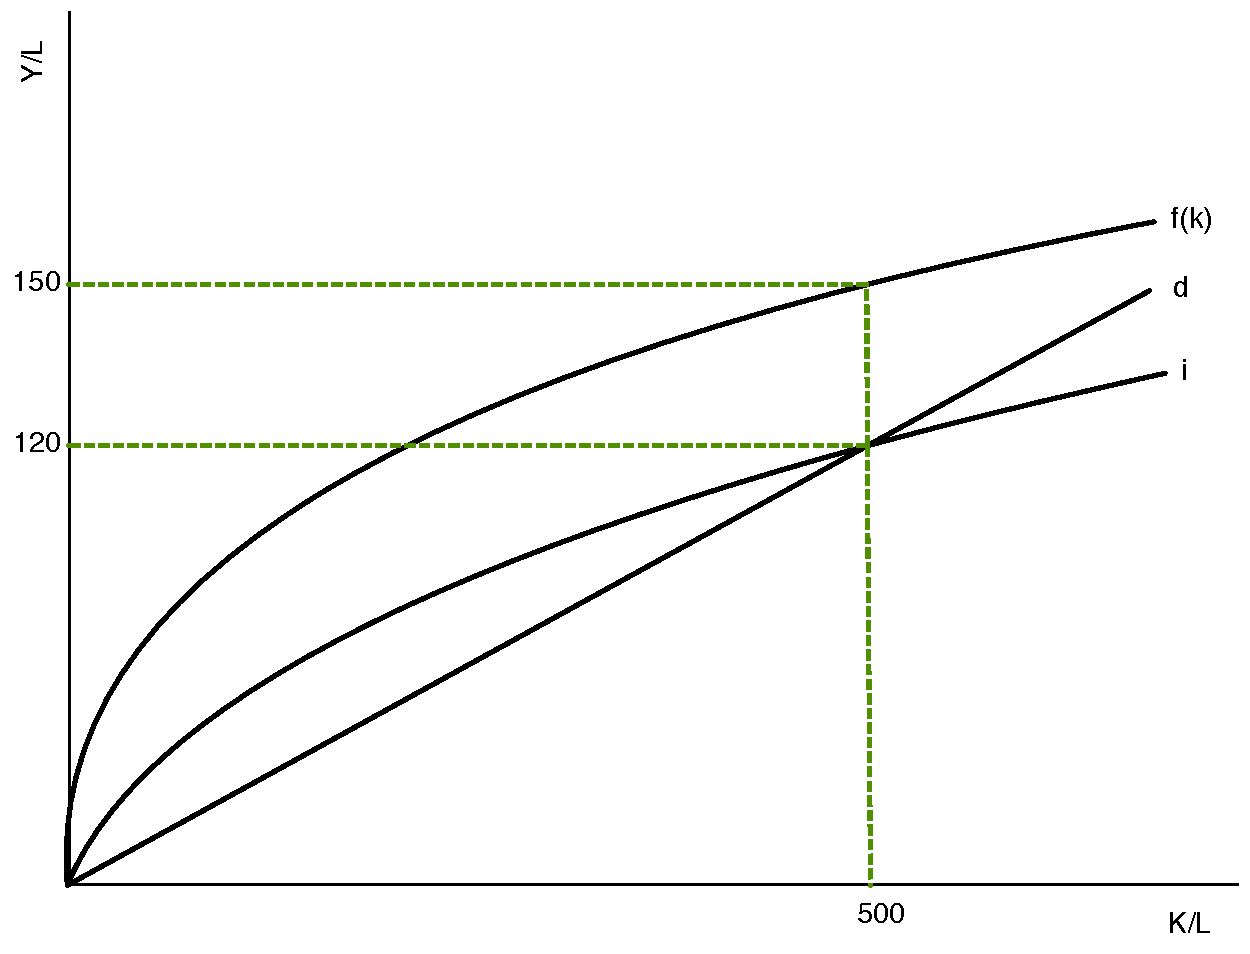
\includegraphics[scale=.4]{Exam2_MC30.pdf}
				\caption{Production in Iceland}
				\label{MC30}
			\end{figure}
			
			The amount of capital per worker that depreciates each period in the steady state is \\ \blank and the percent of output per worker that is consumed in the steady state is \blank.
			
			\begin{choices}
				\choice 500; 80\%
				\CorrectChoice 120; 20\%
				\choice 500; 20\%
				\choice 120; 80\%
			\end{choices}
			
			\begin{solution}
				Steady state where $i=d$. Steady state level of capital is 500, investment is 120, output is 150, and consumption is $150-120=30$. $d^* = i^* = 120$. Percent of output consumed = 30/150 = 20\%.
			\end{solution}
		
		
\end{questions}


\section*{Short Answer}

\begin{questions}
	
		
		\question Table \ref{tab1} shows some data from the land of milk and honey. 
		
		\begin{table}[ht]
			\centering
			\caption{Land of Milk and Honey}
			\label{tab1}
			\begin{tabular}{  c| c | c | c |c}        
				
				Year & Price of Milk & Quantity of Milk & Price of Honey & Quantity of Honey   \\
				\hline
			2013 & \$1 & 100 quarts & \$2 & 50 quarts \\
			2014 & \$1 & 200 & \$2 & 100 \\
			2015 & \$2 & 200 & \$4 & 100 \\
			\end{tabular}
		\end{table} 
		
		\begin{parts}
			\part[6] Compute the nominal and real GDP for each year, using 2013 as the base year. 
			
			\begin{solution}
				Nominal GDP$_t$ = $\sum P_t \cdot Q_t$, real GDP$_t = \sum P_{base yr.}\cdot Q_t$. \\
				2013: $Y^N$ = \$1(100) + \$2(50) = \$200. $Y^R$ = \$1(100) + \$2(50) = \$200.\\
				2014: $Y^N$ = \$1(200) + \$2(100) = \$400. $Y^R$ = \$1(200) + \$2(100) = \$400. \\
				2015: $Y^N$ = \$2(200) + \$4(100) = \$800. $Y^R$ = \$1(200) + \$2(100) = \$400.
			\end{solution}
			
			\part[4] Compute the percentage change in nominal and real GDP in 2014 and 2015. 
			
			\begin{solution}
				$\widehat{Y^N}_{2014} = (400 - 200)/200 = 100\%$. $\widehat{Y^N}_{2015} = (800-400)/400 = 100\%$. \\
				$\widehat{Y^R}_{2014} = (400 - 200)/200 = 100\%$. $\widehat{Y^R}_{2015} = (400-400)/400 = 0\%$.
			\end{solution}
			
			\part[2] Did economic well-being rise more in 2014 or 2015? Explain. 
			
			\begin{solution}
				Real GDP is a better measure of economic well-being. It increased by more in 2014, so well-being rose more in 2014.
			\end{solution}
		\end{parts}

			\question Table \ref{tab2} refers to a small economy that produces two goods - books and calculators. A typical basket of books and calculators consists of 10 books and 2 calculators.
			
			\begin{table}[H]
				\caption{Books and Calculators}
				\label{tab2}
				\centering
				\begin{tabular}{  c|c|c}        
					
					Year   & Price of Books & Price of Calculators \\
					\hline
					2010 &  \$30 & \$4.00\\
					2011 & \$35 & \$4.50\\
					2012 & \$35 & \$6.00 \\
				\end{tabular}
			\end{table}
			\begin{parts}
				\part[3] Calculate the consumer price index for each year, using 2012 as the base year. 
				
				\begin{solution}
					Basket: 10 books, 2 calculators remains fixed. \\
					$P_{2010} = 10\times \$30 + 2\times \$4 = \$308$\\
					$P_{2011} = 10\times \$35 + 2\times \$4.50 = \$359$ \\
					$P_{2012} = 10\times \$35 + 2\times \$6 = \$362$ \\
					CPI$_t$ = $P_t/P_{base yr.}\times 100$. \\
					CPI$_{2010} = (308/362)\times 100 = 85.1$ \\
					CPI$_{2011} = (359/362)\times 100 = 99.2$ \\
					CPI$_{2012} = (362/362)\times 100 = 85.1$ 
				\end{solution}
				
				\part[2] Calculate the inflation rate for 2011 and 2012. 
				
					\begin{solution}
						$\pi_{2011} = (99.2-85.1)/85.1 = 16.57\%.$ \\
						$\pi_{2012} = (100-99.2)/99.2 = .81\%.$ 
					\end{solution}
					
				\part[4] The average salary of a plumber in 2010 was \$22,500, while in 2012 the average salary was \$24,975. Were plumbers better off in 2012 relative to 2010? Explain why. 
				
				\begin{solution}
					2010 salary in 2012 dollars = \$22,500 $\times$ (100/85.1) = \$26,439.48. Plumbers were better off in 2010 (salaries increased by 11\%, but prices increased by approximately 17\% $\Rightarrow$ purchasing power decreased.)
				\end{solution}
				
			\end{parts}
			
			\question A country has the production function $F(K,L) = A K^\beta L^{1-\beta}$, where $0<\beta<1$, $K$ represents the country's capital stock, and $L$ represents its labor force. 
			\begin{parts}
				\part[4] Show that doubling both inputs will double the output the country can produce (i.e., show that $F(2K,2L) = 2F(K,L))$. What is this property called?\footnote{\textbf{Hint:} A couple of properties of exponents are that $x^a\cdot
					 x^{1-a} = x^{(a+1-a)}$ and $(xy)^a = x^a\cdot y^a$.} 
					
				\begin{solution}
					$F(2K,2L) = A(2K)^\beta(2L)^{1-\beta} = A(2)^\beta(2)^{1-\beta}K^\beta L^{1-\beta} = 2^{\beta + 1 - \beta} AK^\beta L^{1-\beta} = 2(AK^\beta L^{1-\beta}) = 2F(K,L)$. This production function exhibits constant returns to scale.
				\end{solution}
				
				\part[6] Define $k = K/L$ as the capital-labor ratio and write output per worker as $f(k) = Ak^\beta$. Suppose $A = 4$ and $\beta = 1/2$. What is the marginal product of capital per worker for the first unit of capital? The second? Third? What property does this show? 
				\begin{solution}
					$Y/L = (1/L)F(K,L) = F(K/L, L/L) = Ak^\beta \equiv f(k)$. Plugging in $A=4$ and $\beta = 1/2$, $f(k) = 4\sqrt{k}$. \\
					$f(0) = 4\sqrt{0} = 0$. \\
					$f(1) = 4\sqrt{1} = 4$. $MP_k = 4-0=4$. \\
					$f(2) = 4\sqrt{2} = 5.66$. $MP_k = 5.66-4 = 1.66$.\\
					$f(3) = 4\sqrt{3} = 6.93$. $MP_k = 6.93-5.66 = 1.27$. \\
					This production function exhibits diminishing marginal returns to capital.
				\end{solution}
				
				\part[6] The capital stock in this country depreciates at rate $\delta=3\%$, output is invested at rate $s=15\%$, and the labor force grows at rate $n=2\%$. It currently has a capital stock per worker of $k_0 = 100$. How much, if any, capital per worker do you expect the country to accumulate (or decumulate) in the long run (i.e., compare the current level of capital to the steady state level of capital)?
				
				\begin{solution}
					$i = sy = .15(4\sqrt{k}) = .6\sqrt{k}$. $d=(n+\delta)k = (.02+.03)k = .05k$. SS: $.6\sqrt{k} = .05k \Rightarrow (.6)^2(\sqrt{k})^2 = (.05)^2k^2 \Rightarrow .36k = .0025k^2 \Rightarrow k^* = (.36/.0025) = 144$. Since capital is currently 100, we expect 44 units of capital to accumulate.
				\end{solution}
				
				\part[3] What is the steady state level of output, investment, and consumption in this country? 
				
				\begin{solution}
					$y* = f(k^*) = 4\sqrt{144} = 48$. \\
					$i^* =sy^* = .15(48) = 7.2$ \\
					$c^* = (1-s)y^* = y^* - i^* = 40.8$.
				\end{solution}
			\end{parts}
		
		\question What topics or questions gave you the most trouble on this homework assignment or the class material it encompassed? 
\end{questions}


\end{document}